\chapter{Project Management}
The following sections details the project management decisions of the project. This includes choice of development method, team member responsibilities, communication channels and risk analysis.

\section{Development method}
\label{development-method}
Based on the customer requirement of short iterations, it was early decided to adapt an iterative and incremental development method for the project. By working in an iterative manner, it was possible to present prototypes and work done to the customer every week, and at the same time receive feedback. In this fashion it was possible for the customer to continuously present his thoughts on the product, and propose changes where he thought it was necessary. The iterative approach on the project also made it easier for the group to set deadlines and milestones of specific parts of the product.\\
\newline
All the members of the group have taken the course TDT4140 - Systemutvikling, and therefore have some knowledge about different development methods. The Rational Unified Process (RUP) model, as described in Chapter~\ref{prestudy} - Prestudy, is an extensible framework\cite{kruchten} that met the requirements the group had for a process model. RUP was chosen as process model for the project above the other models described in Chapter~\ref{prestudy} as it best met the needs of the group. The fact that the model was tailorable and divided the entire development process into phases that was easy to adapt to made it preferable to the other models examined. It was also appealing that the model required the team to focus on critical risks early in the development to avoid surprises.

\subsection{Changes to description}
As mentioned above, it was clear that the use of an iterative model was in order. The specific documentation of the development method was deferred for three weeks, however. This was due to the uncertain future of the project (over the air installation was said to potentially be impossible) and the need to get the first iteration presented to the customer; precisely documenting the development method was deemed to be wasteful at that point in time. The development method description was also refined between the preliminary version and the midterm version of the report.\\
\newline
It was decided to adopt RUP as process model, though with some minor changes. First of all, the Transition phase of the model was deemed unnecessary. This was mainly due to the lack of time and resources for beta testing and new versions of the product. This phase was instead replaced by the closeout phase, described in chapter~\ref{projectplanning}. Further, no cost estimates were developed for the project. Because no money were involved in the production of the product, this was also deemed unnecessary. Time and resource estimates, however, were established during the Inception phase. \\
\newline
In addition to the changes mentioned above, use of Lean principles was adapted from the start of the project. As described in the section about Lean Software Development, this methodology is defined by seven principles. Of these, especially \emph{Eliminate waste} and \emph{Build integrity} were used actively by the team during the development of the product and project report. These principles is described in chapter~\ref{leandev}.

\section{Team roles}
The group was organized in different roles based on skill and experience. Each team member was given a responsibility for some code-packages. Further, the team was divided into six subgroups where each member was held responsible for his or her group. These groups was respectively: group leader, documentation and substitute leader, Android and GUI, Arduino$\texttrademark$ and PUI, over the air and test.
The distribution of team roles are listed in Table~\ref{table:teamroles}

\subsection{Role description}
The division of the group was an important feature. Every member knew who to contact about a specific problem or task.\\

\begin{description}
	\item[Group leader]{was responsible for the progress in the overall project. This person ensured progress and priorities for deadlines.}
	\item[Documentation and substitute leader]{was responsible for management of documentation and reports. In absence of the group leader, this person took on the group leader's responsibilities. This person was also responsible for contact with the customer and supervisor.}
	\item[Android and GUI developer]{was responsible for the Android development of the project.}
	\item[Arduino$\texttrademark$ and PUI developer]{was responsible for the Arduino$\texttrademark$ part of the project. This implies contacting the Arduino$\texttrademark$-lab, requisitions for hardware, the coding part and over-the-air installation. This role was also responsible for development of the PUI examples.}
	\item[Over the air developer]{was responsible for programming the Arduino$\texttrademark$ over the air. This person was also responsible for making the first prototype with a Bluetooth$\textsuperscript{\textregistered}$  connection.}
	\item[Test developer]{was responsible for developing and executing tests for the complete project.}
\end{description}

\begin{table}[H]
\captionof{table}{Roles}
\centering
\label{table:teamroles}
\begin{tabular}{|l|l|}
\hline
	{\bf Name} & {\bf Role}\\
\hline
	Jeppe Benterud Eriksen & Group leader\\
\hline
	Nina Margrethe Smørsgård & Documentation and substitute leader\\
\hline
	Robin Tordly & Android and GUI developer\\
\hline
	Bjørn Arve Fossum & Arduino$\texttrademark$ and PUI developer\\
\hline
	Ståle Semb Hauknes & Over the air developer\\
\hline
	Wilhelm Walberg Schive & Test developer\\
\hline
\end{tabular}
\end{table}

\subsection{Division of Labor}
The division of labor between the members of the group was largely done through the use of issues on GitHub (page \pageref{GitHub}). On this site, whenever a task arose, it was created as an issue. This way, all the members could see what needed to be done, assign different issues to themselves, see what others were working on and therefore choose an appropriate issue to start working on.

Throughout the project the main consensus of the group has been to meet every day as long as there is not something else interfering. This has caused the group to work together almost every day and thus if a problem was met it could be dealt with quickly. Usually these meeting started at 09:00-10:00 and ended around 16:00. Any and all work done by anyone was registered in a document to ensure correct activity plans.

\section{Communication}
Most of the communication within the group was done at group meetings and when the group was working together. For communication between group members outside the meetings it was decided that the group should only use email and Skype. This was decided to avoid the confusion that might arise from using numerous channels of communication. Mobile phone was also used when immediate contact was necessary.\\
\newline
% What about GitHub?
Communication between the group and the customer was mainly done in meetings or by email. The same applies for communication with the supervisor.

\section{Project planning}

\label{projectplanning}

In this section the planning of the project will be presented. The project was divided into five large milestones to represent the different phases of the project. The phases of the Rational Unified Process (RUP) is not explicitly stated in the work breakdown structure, as some of the milestones stretches over several of the phases in the process model. \\
\newline
In the work breakdown structure (WBS), the first part of the Project Management activity and the Planning activity represents the inception and elaboration phase of RUP. Further, the Execution and Testing activities represents the construction phase. As mentioned above the transition phase of RUP was deemed unnecessary. It was expected that tasks related to project management would appear at least until the technical part of the project was concluded, and it was therefore decided to let this activity run through the larger part of the project. In the closeout phase work on the final report was to be prioritized.

\subsection{Work breakdown structure (WBS)}
The WBS is a view on what work packages the project encompasses. It helps with communicating the work and processes to easily execute the project. The duration-time show how much estimated time one task requires, and gives an assessment on how much effort is needed to complete the task.

\subsubsection{Gantt chart}
Gantt chart showing the initial work breakdown structure created in the project.
\begin{figure}[H]
\makebox[\textwidth][c]{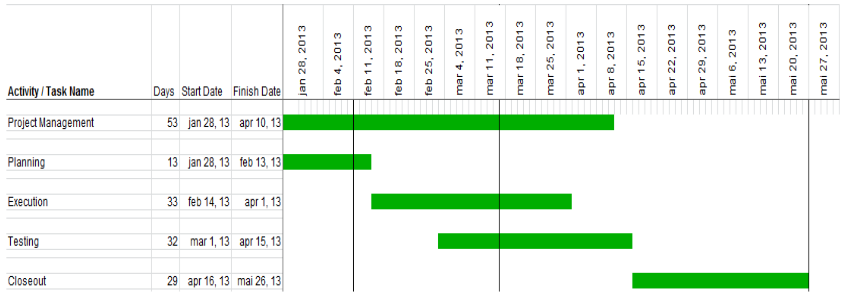
\includegraphics[width=1.2\textwidth]{images/gantt-diagram.png}}
\caption{Gantt chart. Milestones are marked using vertical lines}
\end{figure}

\subsubsection{Work breakdown structure table (WBS table)}
Table~\ref{fig:wbstable} is showing a detailed overview of all the tasks to be preformed in each of the milestones. The WBS code of each task is used to relate it to the WBS tree shown below. This table also contains a description of each task.

\begin{longtable}{|m{0.1 \textwidth}|m{0.1 \textwidth}|m{0.2 \textwidth}|m{0.35\textwidth}|m{0.15 \textwidth}|}
\hline
	\rowcolor{Gray}
	\textbf{Level} & \textbf{WBS{ }Code} & \textbf{Element name} & \textbf{Definition} & \textbf{Duration}\\
	\endfirsthead% 
	\multicolumn{5}{l}%
	{{\bfseries Continued from previous page}} \\ \hline
	\rowcolor{Gray}
	\textbf{Level} & \textbf{WBS{ }Code} & \textbf{Element name} & \textbf{Definition} & \textbf{Duration}\\
\hline
	\endhead%
	\hline
 
	\hline \multicolumn{5}{|l|}{{Continued on next page}} \\ \hline
	\endfoot%
 
	\endlastfoot%

	1 & 1 & $\mu$C Software Store & All work to implement an application store for Arduinos and over the air innstallation with two example PUIs & \\
\hline
	2 & 1.1 & Project management & The work to initiate the project and distribute responsibilities & \\
\hline
	3 & 1.1.1 & Meetings with customer & Determine the project status and decide on requirements & \\
	 & 1.1.2 & Demonstration and play for the customer of the team's understanding of the requirements & Project team evaluates and proposes recommendations & \\
\hline
	 & 1.1.3 & Risk management & Creating risk analysis and agreements within the group and the project & \\
\hline
	 & 1.1.4 & Status report & Write the status report & \\
\hline
	2 & 1.2 & Planning & & \\
\hline
	3 & 1.2.1 & Requirements specification & & \\
\hline
	 & 1.2.2 & Determine Project team & Give each menber a role and distribute tasks & \\
\hline
	 & 1.2.3 & Supervisor meeting & Meeting wih supervisor for instruction and guidance & \\
\hline
	 & 1.2.4 & Develop project plan and use cases & & \\
\hline
	 & 1.2.5 & Research & & \\
\hline
	 & 1.2.5.1 & Research on over the air innstallation & Do research on bluetooth installation on arduinos & \\
\hline
	 & 1.2.5.2 & Research UbiCollab libraries & & \\
\hline
	2 & 1.3 & Execution & Programming and execution of the project & \\
\hline
	3 & 1.3.1 & Project kickoff meeting & First meeting with customer to evaluate knowledge and agree on further meetings & \\
\hline
	 & 1.3.2 & Verify \& validate user requirements & Determine whether the group is in tune with the customers vision of the project requirements & \\
\hline
	 & 1.3.3 & Design system & & \\
\hline	  
	 & 1.3.4 & & & \\
\hline
	 & 1.3.5 & Produce Software & & \\
\hline
	 & 1.3.6 & Instalation over the air implementation & & \\
\hline
	 & 1.3.7 & Documentation & & \\
\hline
	2 & 1.4 & Testing & & \\
\hline
	3 & 1.4.1 & Develop unit tests & & \\
\hline
	 & 1.4.2 & User testing & & \\
\hline
	 & 1.4.3 & Stress testing & & \\
\hline
	 & 1.4.4 & System Testing & & \\
\hline
	2 & 1.5 & Closeout & & \\
\hline
	3 & 1.5.1 & Creating final project report & & \\
\hline
	 & 1.5.2 & Delivery to customer & & \\
\hline
\end{longtable}
\captionof{table}{Work Breakdown Structure}


\subsubsection{Work breakdown structure tree (WBS tree)}
This is the WBS tree made for this specific project.
\begin{figure}[H]
\vspace*{-1.5in}
\hspace*{-1.2in}
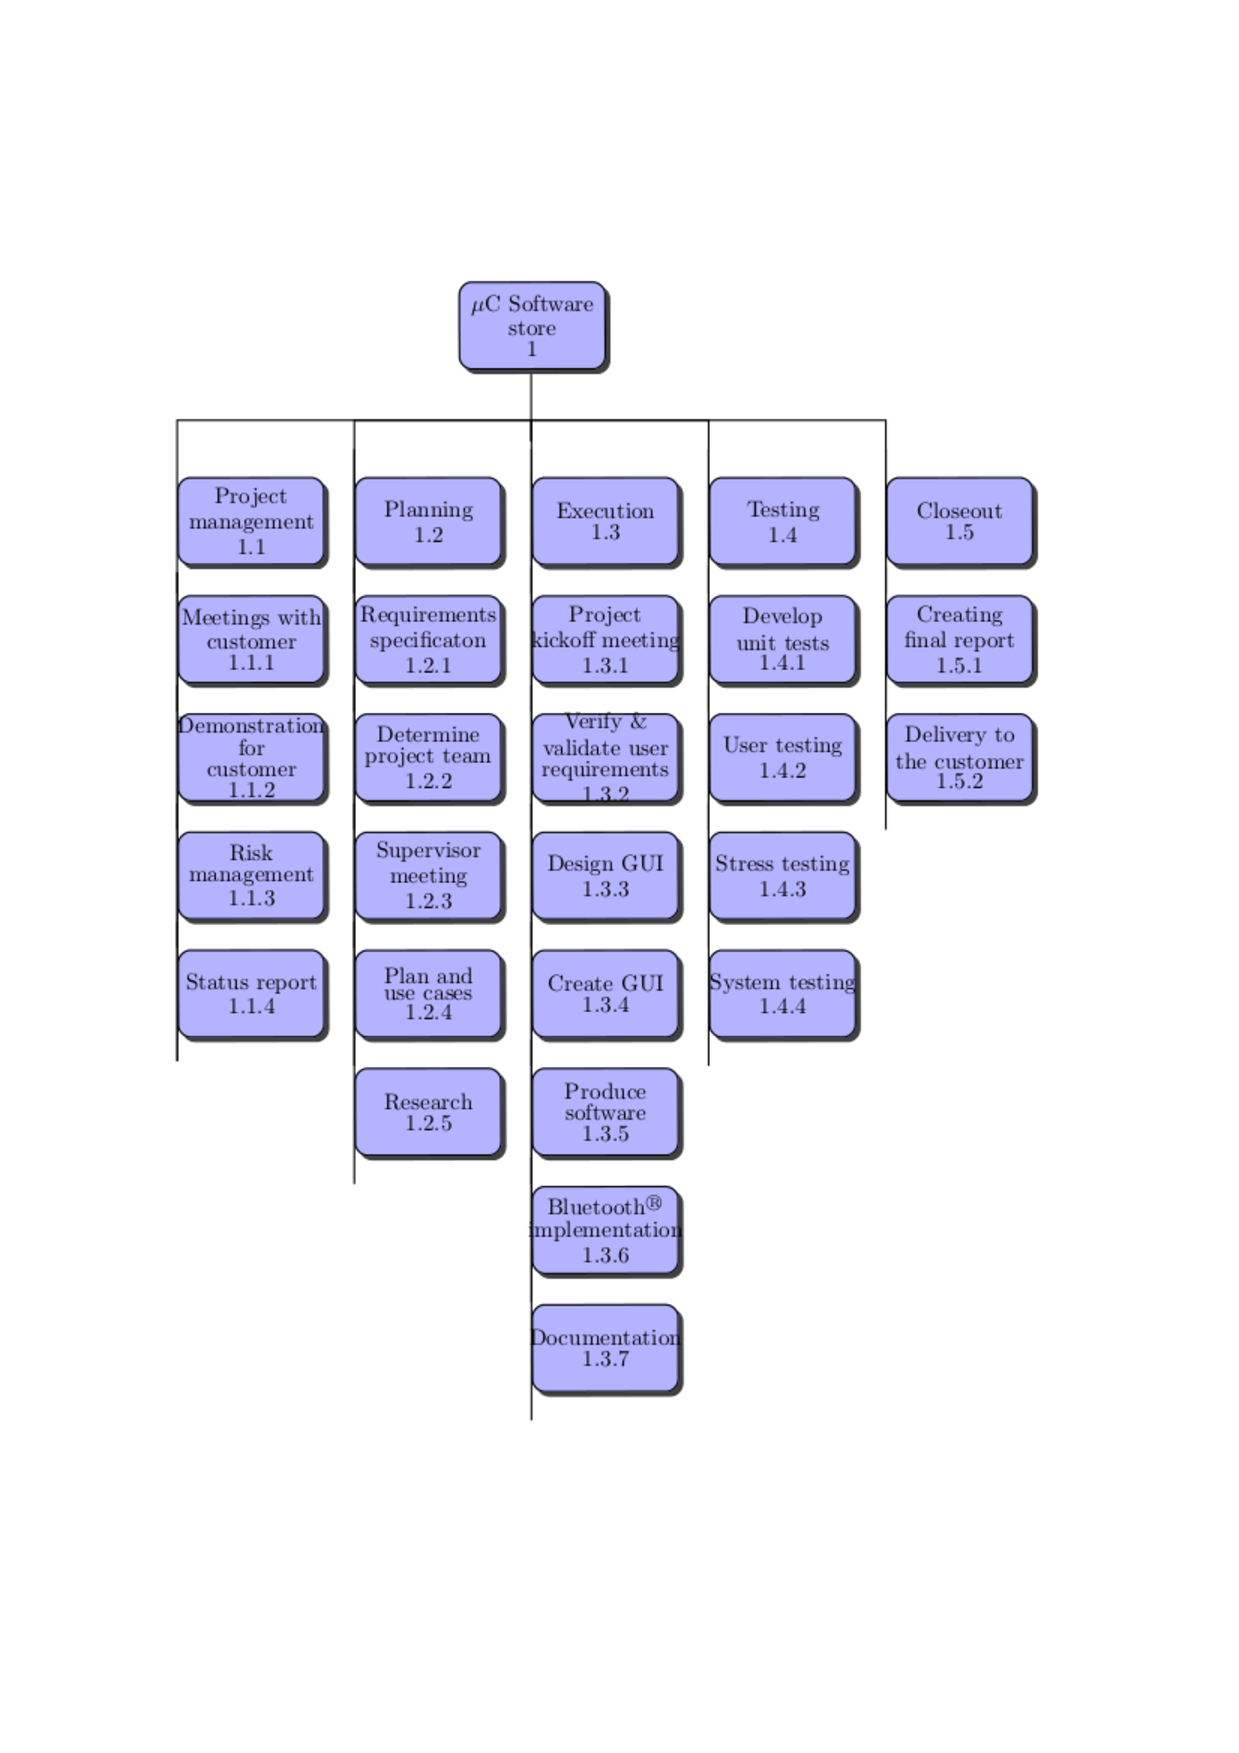
\includegraphics[trim=0cm 4cm 0cm 0cm]{figures/wbs-tree2.pdf}
\captionof{figure}{WBS tree showing a more detailed overview of the different tasks in each of the five milestones.}
\end{figure}

\subsection{Editions to WBS}
Due to challenges and unexpected work that emerged during the project, it was not possible to follow the WBS completely. First of all, a lot of unplanned work arose in connection with the implementation of STK500 in Java. The result of this was that not all group members were able to move to the closeout phase at the same time, as there still was unfinished work on the protocol.

\section{Risk analysis}
The risk analysis as shown in table~\ref{fig:risktable} states risks identified by the team. The importance of a risk is calculated by multiplying likelihood and impact. Higher number means higher importance for the project.
\captionof{table}{Risk analysis}
\label{fig:risktable}
\begin{longtable}{|m{0.15 \textwidth}|m{0.1 \textwidth}|m{0.1 \textwidth}|m{0.1 \textwidth}|m{0.185 \textwidth}|m{0.185 \textwidth}|}
\hline
	\rowcolor{Gray}
	\textbf{Description} & \textbf{Likeli{-}hood} & \textbf{Impact} & \textbf{Impor{-}tance} & \textbf{Preventive\newline Action} & \textbf{Remedial\newline Action}\\
	\endfirsthead%
	\multicolumn{6}{l}%
	{{\bfseries Continued from previous page}} \\ \hline
	\rowcolor{Gray}
	\textbf{Description} & \textbf{Likeli{-}hood} & \textbf{Impact} & \textbf{Impor{-}tance} & \textbf{Preventive\newline Action} & \textbf{Remedial\newline Action}\\
\hline
	\endhead%
	\hline

	\hline \multicolumn{6}{|l|}{{Continued on next page}} \\ \hline
	\endfoot%

	\endlastfoot%

	Illness & 7 & 2 & 14 & Good\newline communication and effective use of GitHub & Increase workhours and exchange tasks and\newline responsibilities\\
\hline
	Project\newline complexity & 6 & 5 & 30 & Don't take on too much work & Cut down the demands\\
\hline
	Customer\newline issues & 1 & 5 & 5 & Agreement with customer and weekly feedback from customer & Use the\newline original\newline requirement specification\\
\hline
	License\newline incompability & 7 & 7 & 49 & Avoid\newline integrating components with incopatible licenses & Discover other implementations or implment from scratch\\
\hline
	Group\newline conflicts or disagreements & 3 & 3 & 9 & Keep close\newline contact to avoid\newline surprises.\newline Leader takes\newline action & Contact\newline supervisor and make an\newline appointment\\
\hline
	Over the air complexity & 8 & 8 & 64 & Have multiple\newline alternative\newline solutions and keep close\newline contact with customer & Detail what was attempted as well as why it couldn't be solved in the final report.\\
\hline
	Personal matters & 8 & 5 & 40 & Not much\newline preventative action can be taken & Keep in touch and stay\newline updated. In case you still can do tasks, claim one and tell the\newline others\\
\hline
\end{longtable}
